\documentclass{ctexart}
\usepackage{graphicx}
\usepackage{amsmath}
\usepackage{amsthm}
\usepackage{amssymb}
\usepackage{fancyhdr}
\usepackage{ifthen}
\usepackage{syntonly}
\usepackage[colorlinks, CJKbookmarks=true, linkcolor=red]{hyperref}
\pagestyle{plain}
\usepackage[raggedright]{titlesec}
\newtheorem{性质}{性质}
\newtheorem{定理}{定理}
\newtheorem{推论}{推论}
\begin{document}
\title{作业}
\author{计算机科学与技术系52班 杨定澄 \and 学号:2015011274 \and E-mail:892431401@qq.com}
\date{}
\maketitle
\section*{第一题}
\subsection*{(a)}
协方差矩阵是$0.2I$,故最小错误概率的分类器满足:

$w^T(x-x_0) \ge 0$时分为$\omega_1$类。

其中$w=\mu_1-\mu_2,x_0=\frac{\mu_1+\mu_2}{2}-\frac{\sigma^2}{||\mu_1-\mu_2||^2}\ln \frac{P(\omega_1)}{P(\omega_2)}(\mu_1-\mu_2)$

将条件代入并化简后得到结果:

若$x_1+x_2 \le 2.5$,就归为$\omega_1$;否则归为$\omega_2$。
\subsection*{(b)}
\begin{align*}
P(error)&=1  \int_{R_1}P(\omega_2|x)dx+0.5  \int_{R_2}P(\omega_1|x)dx\\
		 &=\int_{R_1}P(\omega_2)P(x|\omega_2)dx+0.5  \int_{R_2}P(\omega_1)P(x|\omega_1)dx
\end{align*}
目的是小化正数$P(error)$,而$P(\omega_1)$和$P(\omega_2)$又是相等的正数,故不用考虑,可以改写为最小化
\begin{align*}
P'=&\int_{R_1}P(x|\omega_2)dx+0.5\int_{R_2}P(x|\omega_1)dx\\
  =&\int_{R_1}P(x|\omega_2)dx+0.5[1-\int_{R_1}P(x|\omega_1)dx]\\
  =&0.5+\int_{R_1}[P(x|\omega_2)-0.5P(x|\omega_1)]dx
\end{align*}

为了使$P'$最小,我们可以这么定义分类器:

当$P(x|\omega_2)-0.5P(x|\omega_1)<0$时,$x \in R_1$;否则$x \in R_2$。

接下来只要解$P(x|\omega_2)-0.5P(x|\omega_1)<0$即可。

\begin{align*}
&P(x|\omega_2)-0.5P(x|\omega_1)<0 \\
\Longrightarrow&	P(\omega_1)>2P(x|\omega_2)\\
\Longrightarrow& \frac{P(\omega_1)}{P(\omega_2)}>2 \\
\Longrightarrow& \ln[\frac{P(\omega_1)}{P(\omega_2)}]>\ln2\\
\Longrightarrow& -\frac{[(x_1-1)^2+(x_2-1)^2]-[(x_1-1.5)^2+(x_2-1.5)^2]}{0.4}<\ln2\\
\Longrightarrow& x_1+x_2<2.5-0.4\ln2
\end{align*}

故在该loss matrix下的分类器是,当$x_1+x_2<2.5-0.4\ln2$时为$\omega_1$,否则为$\omega_2$。
\subsection*{(c)}
我用python实现了一个小程序,就在附件里的classifier.py中。

会分别跑$10$次计算正确率,在第$8$行和第$9$行中可以通过注释选择$\mu_2$为$[1.5,1.5]^T\textrm{还是}[3.0,3.0]^T$。

当$\mu_2=[1.5,1.5]^T$时,一组结果如图

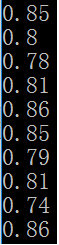
\includegraphics{1.png}

当$\mu_2=[3.0,3.0]^T$时,一组结果如图

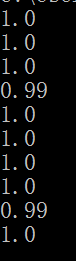
\includegraphics{2.png}

可以看出,第二种情况下,$\mu_1$和$\mu_2$的偏差较大,故该分类器准确率更高。
\section*{第二题}
已知$\int_{R_1}P(\omega_2|x)dx=\epsilon$,要求最小化$\int_{R_2}P(\omega_1|x)dx$。

我们有$\int_{R_2}P(\omega_1|x)dx=1-\int_{R_1}P(\omega_1|x)dx$,故只需要最大化$\int_{R_1}P(\omega_1|x)dx$。

由拉格朗日乘数法知,在满足$\int_{R_1}P(\omega_2|x)dx=\epsilon$下$\int_{R_1}P(\omega_1|x)dx$的最大值,等于$\int_{R_1}P(\omega_1|x)dx+\lambda(\epsilon-\int_{R_1}P(\omega_2|x)dx)=\lambda \epsilon+\int_{R_1}[P(\omega_1|x)-\lambda P(\omega_2|x)]dx$。

很显然,最后的分类方式是,若$P(\omega_1|x)-\lambda P(\omega_2) \ge 0$,就分为$\omega_1$类,否则分为$\omega_2$类。

也即$\frac{P(\omega_1|x)}{P(\omega_2|x)}>\theta$时分为$\omega_1$类。
\section*{第三题}
这道题满足$\sum_i=\sum$,结合$P(\omega_1)=P(\omega_2)=P(\omega_3)$,我们可以用如下方式定义$g_i(x)$。

$g_i(x)=-(x-\mu_i)^T\sum^{-1}(x-\mu_i)$

只需比较三者大小即可。

将所有数据代入原式,用MATLAB计算可知,$g_1(x)=-2.3610,g_2(x)=-0.2410,g_3(x)=-9.4190$。

因此,我们选择将它分类到$\omega_2$类中。
\end{document}
